% Options for packages loaded elsewhere
\PassOptionsToPackage{unicode}{hyperref}
\PassOptionsToPackage{hyphens}{url}
%
\documentclass[
  ignorenonframetext,
  aspectratio=169]{beamer}
\usepackage{pgfpages}
\setbeamertemplate{caption}[numbered]
\setbeamertemplate{caption label separator}{: }
\setbeamercolor{caption name}{fg=normal text.fg}
\beamertemplatenavigationsymbolsempty
% Prevent slide breaks in the middle of a paragraph
\widowpenalties 1 10000
\raggedbottom
\setbeamertemplate{part page}{
  \centering
  \begin{beamercolorbox}[sep=16pt,center]{part title}
    \usebeamerfont{part title}\insertpart\par
  \end{beamercolorbox}
}
\setbeamertemplate{section page}{
  \centering
  \begin{beamercolorbox}[sep=12pt,center]{part title}
    \usebeamerfont{section title}\insertsection\par
  \end{beamercolorbox}
}
\setbeamertemplate{subsection page}{
  \centering
  \begin{beamercolorbox}[sep=8pt,center]{part title}
    \usebeamerfont{subsection title}\insertsubsection\par
  \end{beamercolorbox}
}
\AtBeginPart{
  \frame{\partpage}
}
\AtBeginSection{
  \ifbibliography
  \else
    \frame{\sectionpage}
  \fi
}
\AtBeginSubsection{
  \frame{\subsectionpage}
}
\usepackage{amsmath,amssymb}
\usepackage{lmodern}
\usepackage{iftex}
\ifPDFTeX
  \usepackage[T1]{fontenc}
  \usepackage[utf8]{inputenc}
  \usepackage{textcomp} % provide euro and other symbols
\else % if luatex or xetex
  \usepackage{unicode-math}
  \defaultfontfeatures{Scale=MatchLowercase}
  \defaultfontfeatures[\rmfamily]{Ligatures=TeX,Scale=1}
\fi
\usetheme[]{Frankfurt}
\usecolortheme{beaver}
% Use upquote if available, for straight quotes in verbatim environments
\IfFileExists{upquote.sty}{\usepackage{upquote}}{}
\IfFileExists{microtype.sty}{% use microtype if available
  \usepackage[]{microtype}
  \UseMicrotypeSet[protrusion]{basicmath} % disable protrusion for tt fonts
}{}
\makeatletter
\@ifundefined{KOMAClassName}{% if non-KOMA class
  \IfFileExists{parskip.sty}{%
    \usepackage{parskip}
  }{% else
    \setlength{\parindent}{0pt}
    \setlength{\parskip}{6pt plus 2pt minus 1pt}}
}{% if KOMA class
  \KOMAoptions{parskip=half}}
\makeatother
\usepackage{xcolor}
\newif\ifbibliography
\setlength{\emergencystretch}{3em} % prevent overfull lines
\providecommand{\tightlist}{%
  \setlength{\itemsep}{0pt}\setlength{\parskip}{0pt}}
\setcounter{secnumdepth}{-\maxdimen} % remove section numbering
\usepackage{booktabs}
\usepackage{longtable}
\usepackage{array}
\usepackage{multirow}
\usepackage{wrapfig}
\usepackage{float}
\usepackage{colortbl}
\usepackage{pdflscape}
\usepackage{tabu}
\usepackage{threeparttable}
\usepackage{threeparttablex}
\usepackage[normalem]{ulem}
\usepackage{makecell}
\usepackage{xcolor}
\usepackage{tikz} % required for image opacity change
\usepackage[absolute,overlay]{textpos} % for text formatting

% this font option is amenable for beamer
\setbeamerfont{caption}{size=\tiny}

\newcommand{\bcolumns}{\begin{columns}[T, onlytextwidth]}
\newcommand{\ecolumns}{\end{columns}}

\newcommand{\bdescription}{\begin{description}}
\newcommand{\edescription}{\end{description}}

\newcommand{\bitemize}{\begin{itemize}}
\newcommand{\eitemize}{\end{itemize}}
\AtBeginSubsection{}
\ifLuaTeX
  \usepackage{selnolig}  % disable illegal ligatures
\fi
\usepackage[]{natbib}
\bibliographystyle{plainnat}
\IfFileExists{bookmark.sty}{\usepackage{bookmark}}{\usepackage{hyperref}}
\IfFileExists{xurl.sty}{\usepackage{xurl}}{} % add URL line breaks if available
\urlstyle{same} % disable monospaced font for URLs
\hypersetup{
  pdftitle={Conservation of biodiversity -- current practices national legislation and international conventions and treaties, and biodiversity prospects and intellectual property rights.},
  hidelinks,
  pdfcreator={LaTeX via pandoc}}

\title{Conservation of biodiversity -- current practices national
legislation and international conventions and treaties, and biodiversity
prospects and intellectual property rights.}
\author{Deependra Dhakal\\
Assistant Professor\\
Agriculture and Forestry University\\
\textit{ddhakal.rookie@gmail.com}\\
\url{https://rookie.rbind.io}}
\date{}

\begin{document}
\frame{\titlepage}

\begin{frame}[allowframebreaks]
  \tableofcontents[hideallsubsections]
\end{frame}
\hypertarget{value-of-biodiversity}{%
\section{Value of biodiversity}\label{value-of-biodiversity}}

\begin{frame}{}
\protect\hypertarget{section}{}
\begin{itemize}
\tightlist
\item
  Value based on as anthropocentric/utilitarian appraoch and ecocentric
  approach.
\item
  Utilitarian approach assigns values for

  \begin{itemize}
  \tightlist
  \item
    aesthetics, and
  \item
    the moral responsibility of humanity to preserve natural resources
    (thus as indicator of sustainable use of resource)
  \end{itemize}
\item
  Ecocentric approach is concerned with the intrinsic value of
  biodiversity, meaning its value independent from its contribution to
  human welfare.
\item
  Direct use value as food and medicines, clothing, energy and shelter;
  items of direct use value are privately appropriable.
\item
  80\% of the people in developing countries rely on traditional
  medicine for primary health care needs.
\item
  Indirect use value: ecosystem services and templates for industrial
  products; Regulatory functions of ecosystem, nutrient recycling,
  sedimentation processes, waste treatment, water regulation etc.
\item
  Long term or option value: Value in diversity of amount of
  information, for conservation and natural evolutionary mechanism
  sustainance.
\end{itemize}
\end{frame}

\hypertarget{biodiversity-conservation}{%
\section{Biodiversity conservation}\label{biodiversity-conservation}}

\begin{frame}{Background}
\protect\hypertarget{background}{}
\begin{itemize}
\tightlist
\item
  Conservationists' focus has expanded from the objective of
  establishing beautiful parks and conserving select species towards a
  more holistic goal of ecosystem integrity; a goal that goes well
  beyond the conservation of individual species and beautiful landscapes
  to include the protection of the existing diversity of species,
  natural habitats, and ecosystem processes.
\item
  Fundamental questions about goals and strategies, particularly

  \begin{enumerate}
  \tightlist
  \item
    What biodiversity should be conserved; e.g., should the focus be
    particular species, ecosystems, or ecosystem services?
  \item
    Where does the targeted biodiversity occur, and where is the best
    place to protect it? and
  \item
    Given the variety of conservation tools available, which is the most
    effective method to achieve conservation objectives?
  \end{enumerate}
\end{itemize}
\end{frame}

\begin{frame}{}
\protect\hypertarget{section-1}{}
\begin{itemize}
\tightlist
\item
  Traditional form of contribution to conservation effort due following
  peoples:

  \begin{itemize}
  \tightlist
  \item
    Geographers
  \item
    Ethnobotanists
  \item
    Plant ecologists
  \end{itemize}
\item
  Interplay of physical diversity and human management diversity gives
  rise complexity in agrobiodiversity.
\end{itemize}
\end{frame}

\begin{frame}{Operational considerations}
\protect\hypertarget{operational-considerations}{}
\begin{itemize}
\tightlist
\item
  Hotspots approach to defining what should be conserved or
  coarse-filter/fine-filter approach that ensures that a given
  landscape's naturally occuring species and ecological communities are
  protected.
\item
  Identifying the appropriate conservation landscape scale (Species/taxa
  or spatial scale)
\item
  Need for multiple conservation operational tools (Governance based,
  Market based, Civil society based)
\item
  Economic evaluation and conservation trade-offs with competing
  resource demands
\item
  Use of ``easy'' tools (i.e., GIS models and remote sensing data) to
  resolve ecological features and processes and design interventions.
\end{itemize}
\end{frame}

\hypertarget{causes-of-biodiversity-loss}{%
\section{Causes of biodiversity
loss}\label{causes-of-biodiversity-loss}}

\begin{frame}{Introduction}
\protect\hypertarget{introduction}{}
\begin{itemize}
\tightlist
\item
  It is thought that global biodiversity reached its absolute peak about
  30,000 years ago.
\item
  Antropogenic biodiversity loss is estimated at 100-1000 times higher
  than the estimated rates for natural extinction process.
\item
  Genetic erosion in \emph{in-situ} conservation; In china diversity of
  wheat varieties used have decreased 10 times between 1949 and 1970.
\item
  Contaminiation in regenerating cross-pollinated species.
\item
  Storage conditions and handling in \emph{ex-situ}.
\item
  Restructuring or financial leanness of storage institutions.
\end{itemize}
\end{frame}

\begin{frame}{Major drivers}
\protect\hypertarget{major-drivers}{}
\begin{itemize}
\tightlist
\item
  Habitat loss, overexploitation, alien species introductions, building
  and mechanical constructions, and climate change have resulted in
  significant losses to biodiversity, especially over the past 50 years.
\item
  These drivers are a influential both in protected as well as open
  areas.
\item
  Within protected areas

  \begin{itemize}
  \tightlist
  \item
    range of physical (e.g., fire),
  \item
    biological (e.g., alien species),
  \item
    social (e.g., community opposition),
  \item
    political (e.g., political support),
  \item
    economic (lack of resources), and
  \item
    managerial (e.g., lack of planning) threats are faced by
    biodiversity
  \end{itemize}
\end{itemize}
\end{frame}

\hypertarget{risk-of-extinction-and-recovery-program}{%
\section{Risk of extinction and recovery
program}\label{risk-of-extinction-and-recovery-program}}

\begin{frame}{Risk of extinction}
\protect\hypertarget{risk-of-extinction}{}
\bcolumns
\column{0.6\textwidth}

\begin{itemize}
\tightlist
\item
  During the last 500 million years, Earth experienced five periods of
  \textbf{mass extinction} when at least half the living creatures were
  wiped out.

  \begin{itemize}
  \item Ordovician (445 MYA) -- intense ice age -- 60-70% extinction
  \item Devonian (375-360 MYA) -- drastic drop in oxygen levels -- 75% extinction
  \item Permian (252 MYA) -- Asteriod impacts, intensive volcanic activity -- 95% extinction
  \item Triassic (200 MYA) -- Massive volcanic eruptions, asteriods -- 70-80% extinction
  \item Cretaceous (66 MYA) -- Asteriod impact -- 75% extinction
  \end{itemize}
\end{itemize}

\column{0.4\textwidth}

\begin{center}
\includegraphics[width=0.36\linewidth]{../images/we_was_dinasaurs} \end{center}

\begin{center}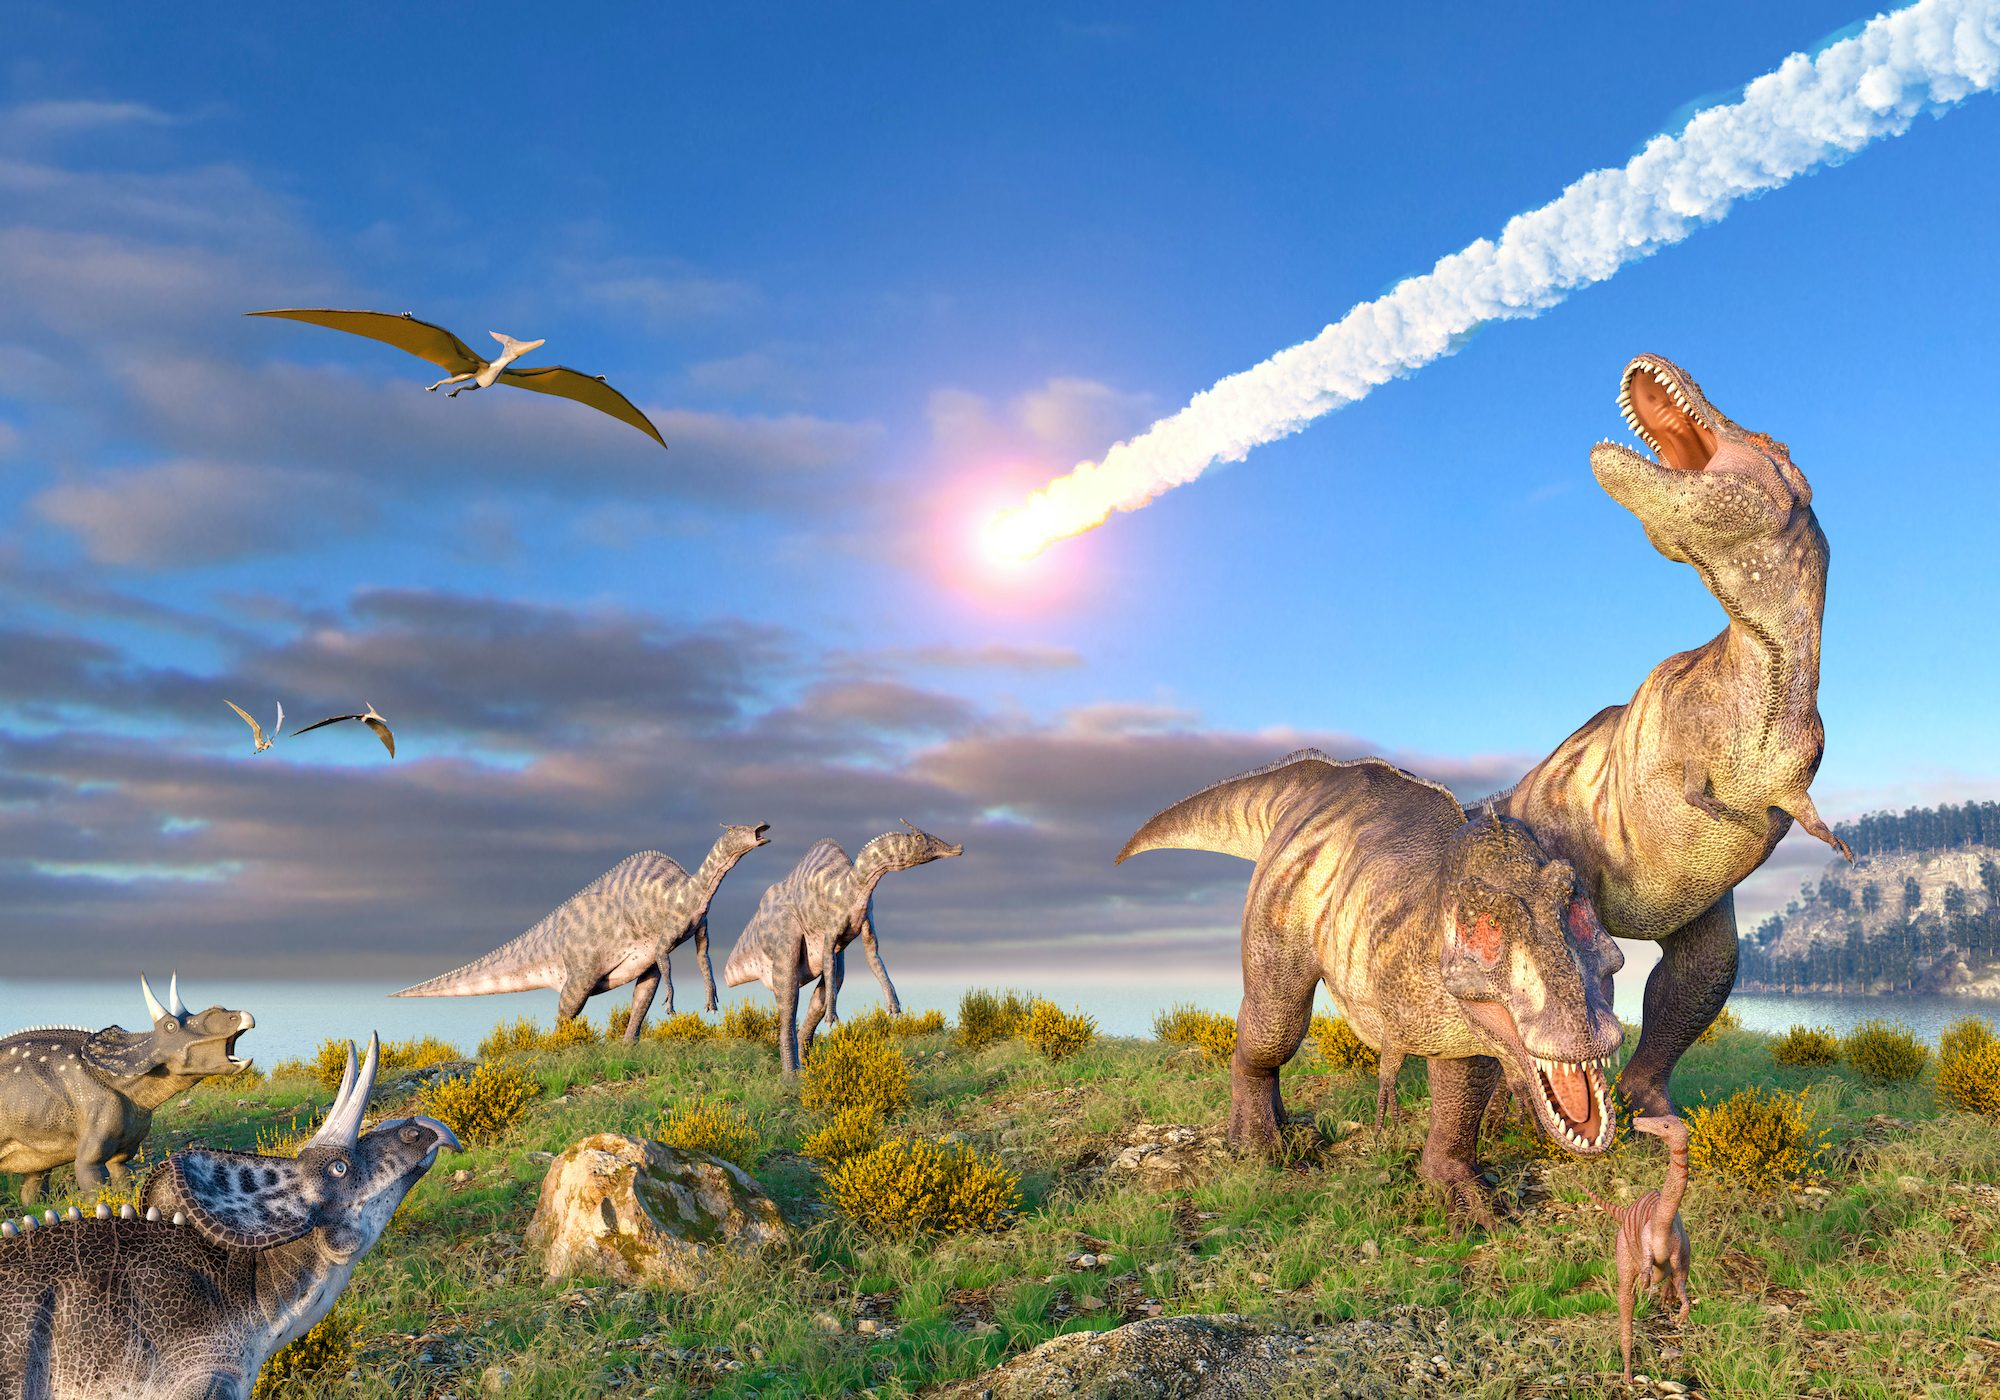
\includegraphics[width=0.98\linewidth]{../images/mass_extinction_illustration} \end{center}

\ecolumns
\end{frame}

\begin{frame}{}
\protect\hypertarget{section-2}{}
\bcolumns
\column{0.6\textwidth}

\begin{itemize}
\tightlist
\item
  \textbf{Occasionally, we should expect to lose many species, whereas
  over most time periods, only a few species should be expected to be
  lost}.
\item
  Therefore, the greater the disturbance, the greater the effect
  (reduction) on biodiversity.
\item
  Probability of species loss depend mostly on:

  \begin{itemize}
  \tightlist
  \item
    Size of the population of species within the community
  \item
    Species with narrow geographic ranges may be more susceptible to
    extinction
  \item
    Small populations exhibit lower genetic variability
  \end{itemize}
\item
  Fossil records, provides the most direct evidence for tracing temporal
  changes in biodiversity, including both the origin and extinction of
  lineages.
\end{itemize}

\column{0.4\textwidth}

\begin{figure}
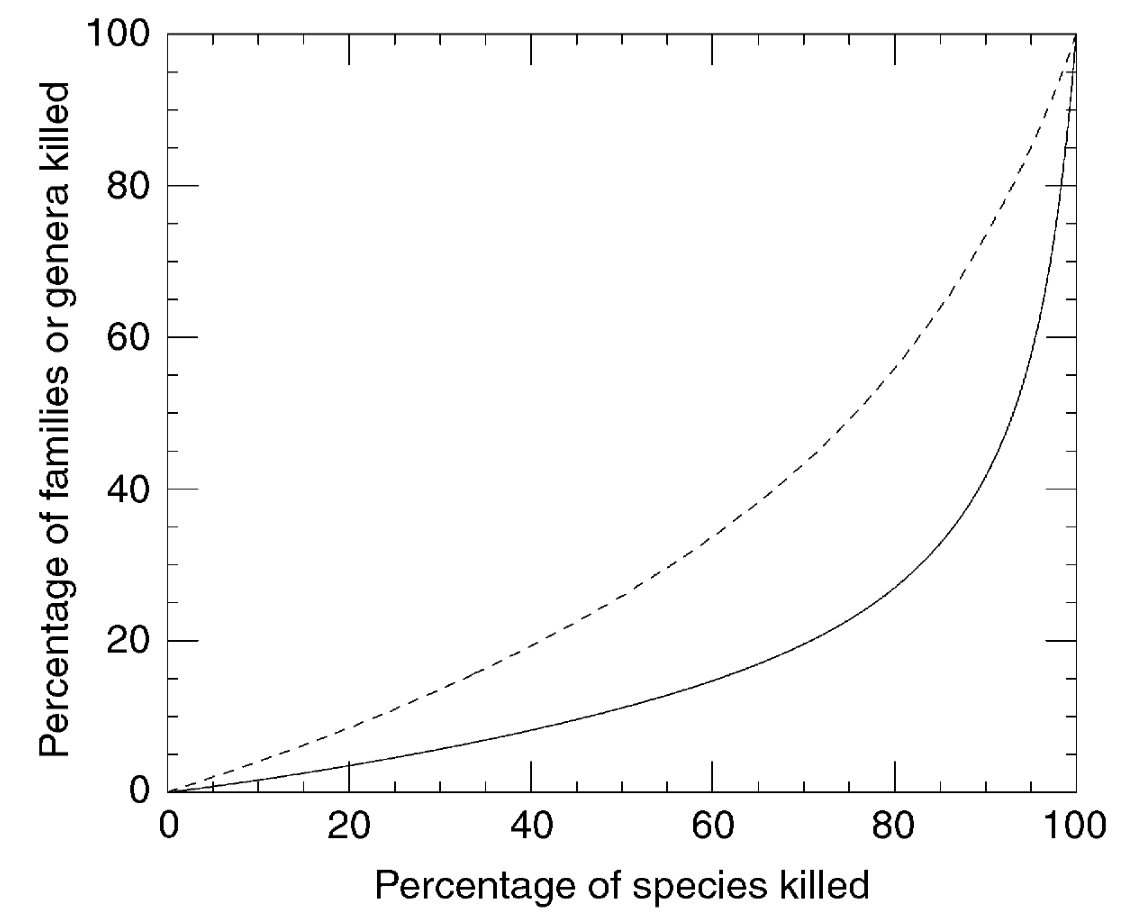
\includegraphics[width=0.7\linewidth]{../images/rarefaction_curve} \caption{Rarefaction curves for the extinction of families (solid line) and genera (dashed line) calculated for echinoderms by Raup (1979). The curves indicate what percentage of families or genera are expected to become extinct during an event which kills a given percentage of species. Used in reverse, the curves also allow us to estimate what percentage of species became extinct in a particular event, given an observed percentage of family or genus kill.}\label{fig:rarefaction-curve}
\end{figure}

\ecolumns
\end{frame}

\begin{frame}{}
\protect\hypertarget{section-3}{}
\bcolumns
\column{0.35\textwidth}
\footnotesize

\begin{itemize}
\tightlist
\item
  It is necessary to evaluate the risk of extinction by determining
  factors such as the absolute abundance of individuals within species
  and how this influences the extinction risk.
\item
  Experimental work on laboratory and field communities suggests that
  decreasing biodiversity also leads to a reduction in ecological time
  of ecosystem function, such as total productivity and carbon dioxide
  sequestration.
\end{itemize}

\column{0.65\textwidth}

\begin{figure}

{\centering 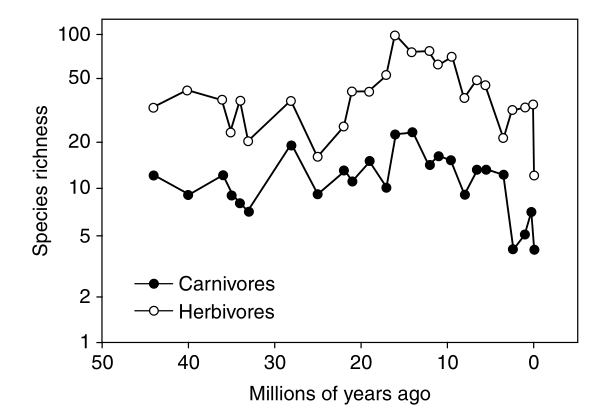
\includegraphics[width=0.5\linewidth]{../images/diversity_of_predatory_prey_history} 

}

\caption{The number of large mammal species from North America during the past 44 million years. Note the correlation between the diversity of predators and their potential prey ($r^2 = 0.43; p < 0.001$)}\label{fig:predator-prey-history}
\end{figure}

\begin{figure}
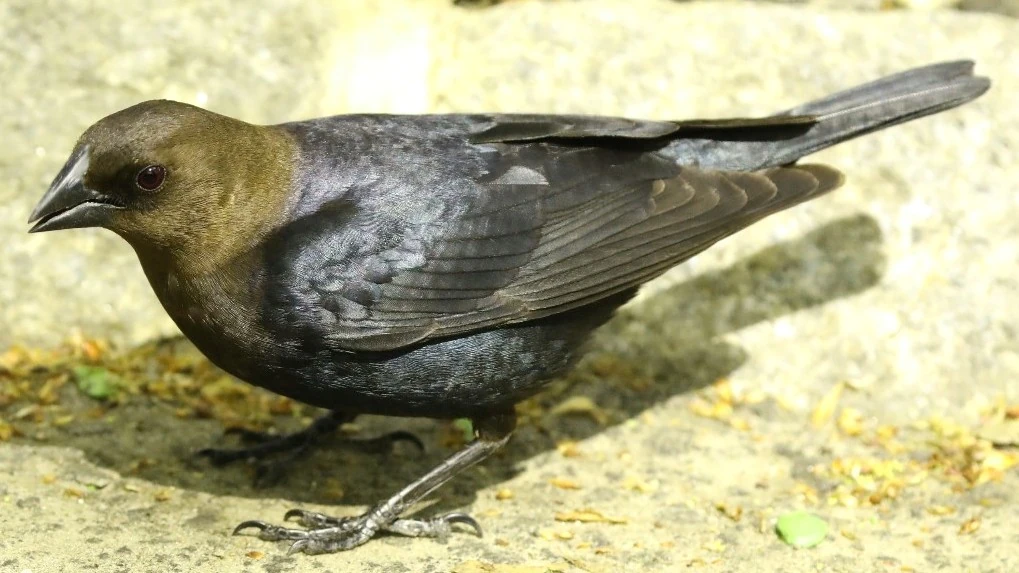
\includegraphics[width=0.5\linewidth]{../images/cowbird} \caption{The convex-billed cowbird (\textit{Pandanaris convexa}) is a species of bird in the family Icteridae, and the only living member of the genus Pandanaris, that originally lived in North America during the Pleistocene. Its extinction was associated with the extinction of large herbivores.}\label{fig:pandanaris-cowbird}
\end{figure}

\ecolumns
\end{frame}

\begin{frame}{}
\protect\hypertarget{section-4}{}
Southeast Asia possesses an estimated vascular flora of around 60,000
species (20,000-25,000 species in Indo-China and 42,000 species in
Malesia). Of 1371 red-listed plant species in Southeast Asia, 292 are
critically endangered, 196 endangered, 737 vulnerable, 31
near-threatened, and 110 data-deficient. Five plant extinctions are
documented: two mangos ( \emph{Mangifera casturi} Kosterm and
\emph{Mangifera rubropetala} Kosterm), two dipterocarp trees (
\emph{Dipterocarpus cinereus} Sloot and \emph{Shorea cuspidata} Ashton),
and one herb - the ``woolly stalked Begonia'' ( \emph{Begonia
eiromischa} Ridl.). Only the mangos survive in ex situ collections
(IUCNRedlist.org, accessed 23 August 2011)

Since AD 1500, at least 132 bird species have gone extinct (EX), and a
further four are extinct in the wild (EW). Strikingly, 121 (92\%) of
these species were confined to islands, mostly in the Pacific, and an
additional three were confined to single lake (Birdlife International,
2011).
\end{frame}

\begin{frame}{Recovery programs}
\protect\hypertarget{recovery-programs}{}
\bcolumns
\column{0.7\textwidth}

\begin{itemize}
\tightlist
\item
  Endangered species are in the most imminent needs of attention for
  recovery (species recovery/conservation plan/action).
\item
  A recovery plan describes the current status, threats and intended
  methods for increasing rare and endangered species.
\item
  The Species Survival Commission's Specialist Groups of the
  International Union for Conservation of Nature (IUCN) has created
  Species Action Plans since at least the mid-1980s, which are used to
  outline the conservation strategies of species, normally between set
  dates.
\item
  Either a single species or an area, habitat or ecosystem or entire
  landscape can be targeted by the recovery plan.
\end{itemize}

\column{0.3\textwidth}

\begin{center}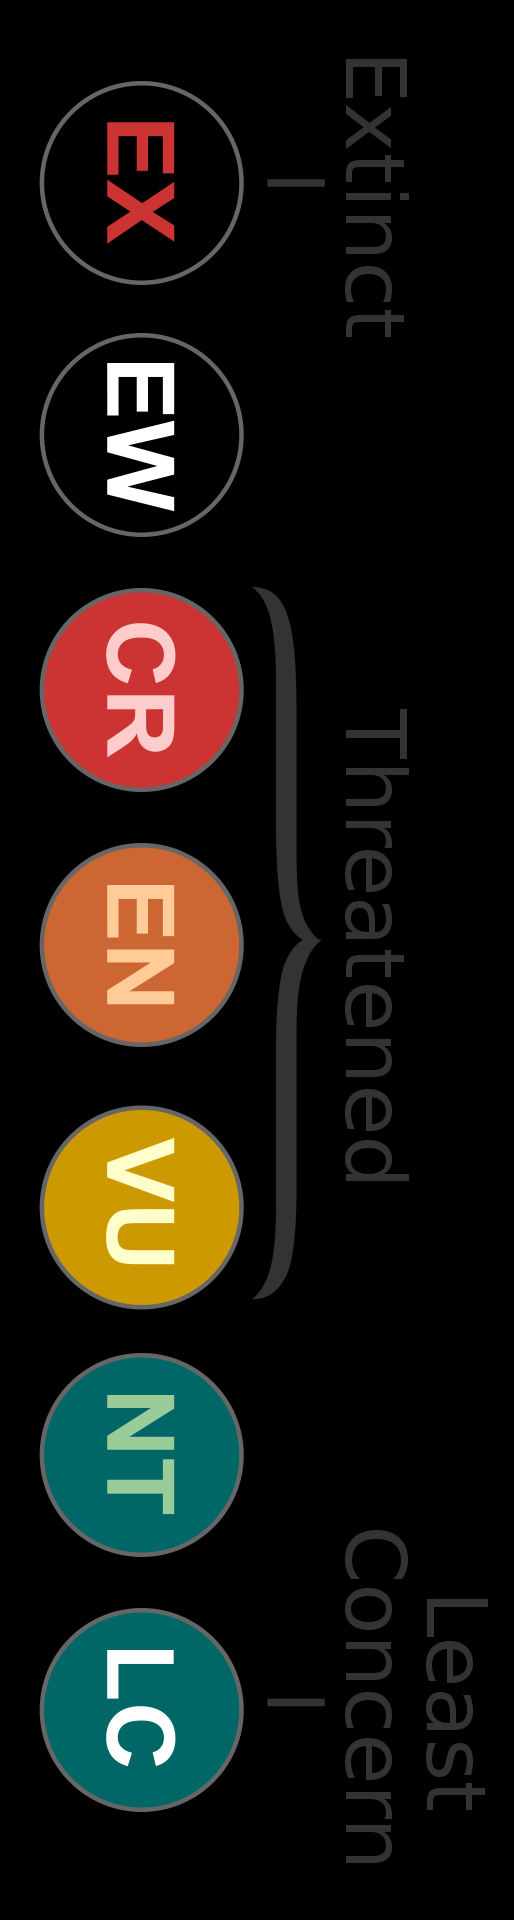
\includegraphics[width=0.4\linewidth]{../images/IUCN_classification} \end{center}

\ecolumns
\end{frame}

\begin{frame}{}
\protect\hypertarget{section-5}{}
\bcolumns
\column{0.5\textwidth}

\begin{center}
\includegraphics[width=0.65\linewidth]{../images/Vulture_conservation_action_plan} \end{center}

\column{0.5\textwidth}

\begin{center}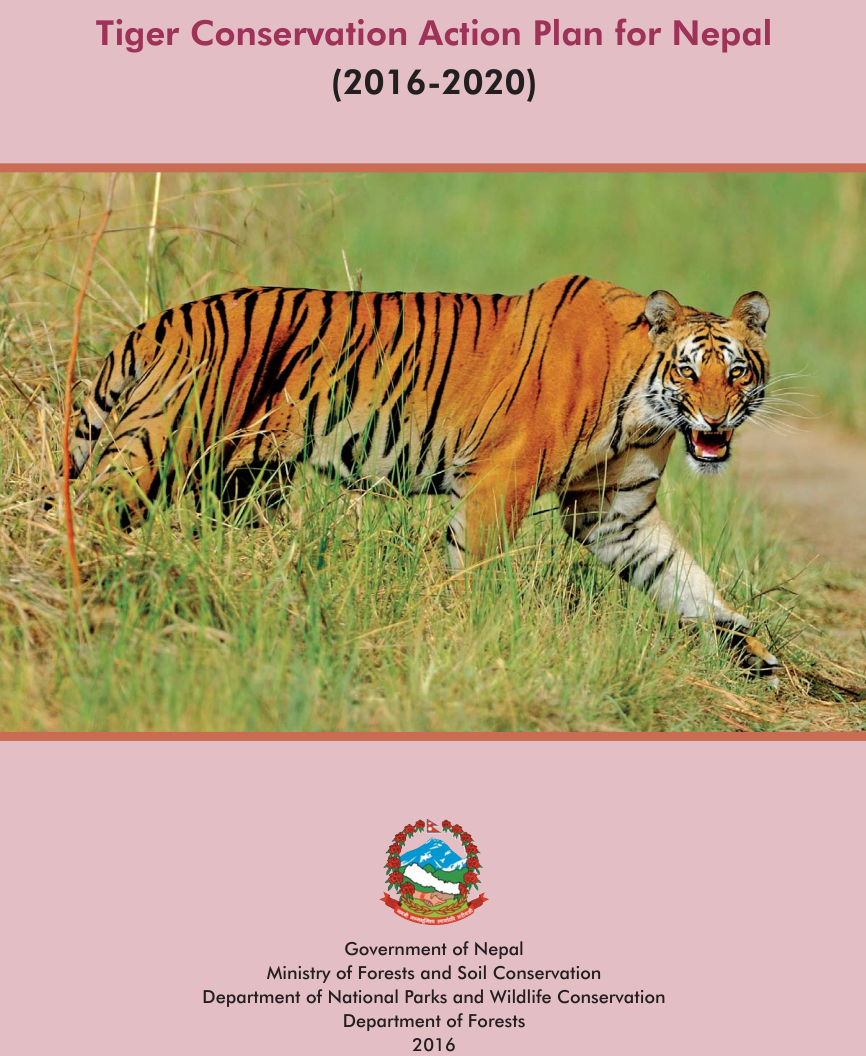
\includegraphics[width=0.48\linewidth]{../images/Tiger_recovery_plan} \end{center}

\ecolumns
\end{frame}

\begin{frame}{}
\protect\hypertarget{section-6}{}
\begin{itemize}
\tightlist
\item
  Recovery program are conducted at both coarse-filter and fine-filter
  approach.
\item
  Coarse filter approach focuses on habitat and most, if not all
  species, and their ecological functions being supported in reserves
  and conservation areas.

  \begin{itemize}
  \tightlist
  \item
    For example in conserving invertebrates (grasshoppers, ants and
    snail) species, a major consideration is that of effor to restore
    stone-cover.
  \end{itemize}
\item
  Restoration of grazing in areas where plant succession eliminates
  savannah-like, open habi tats often results in the increase of the
  species richness of native pollinators and other invertebrates.
\item
  The Lord Howe Island stick insect ( \emph{Dryococelus australis}) had
  been thought to be extinct until a small population was found on a
  tiny Ball's Pyramid Islet (New 2012); a small fraction of the
  population has been collected and is now successfully breeding in
  captivity at Melbourne Zoo.
\end{itemize}
\end{frame}

\begin{frame}{}
\protect\hypertarget{section-7}{}
\footnotesize

\begin{itemize}
\tightlist
\item
  Reintroduction and restocking programs (generally effective for birds)
  may be employed when a wild population is otherwise beyond recovery.
\item
  These programs are decided based on:

  \begin{itemize}
  \tightlist
  \item
    organism's ecology
  \item
    current threats
  \item
    suitability of available stock
  \item
    regional human socio-economic implications
  \end{itemize}
\item
  Release should only take place when the habitat is capable of
  sustaining a viable population and original constraining factors no
  longer operate.
\item
  Proper recovery programs do not simply act as stop gaps to prevent
  extinction, but can restore species to a state of health so they are
  self-sustaining.
\item
  Best plans are adaptive and dynamic, responding to changing
  conditions.
\end{itemize}
\end{frame}

\hypertarget{forms-of-biodiversity-conservation}{%
\section{Forms of biodiversity
conservation}\label{forms-of-biodiversity-conservation}}

\begin{frame}{On farm conservation}
\protect\hypertarget{on-farm-conservation}{}
\begin{itemize}
\tightlist
\item
  Seed preservation by farmer household
\item
  Participatory variety breeding
\item
  Culture based importance for conservation
\end{itemize}
\end{frame}

\begin{frame}{Protected area conservation: History}
\protect\hypertarget{protected-area-conservation-history}{}
\begin{itemize}
\tightlist
\item
  As long as 2000 years ago ancient societies in Greece, Rome, Asia, and
  Africa are known to have set aside areas as sacred groves or sites,
  while european societies had hunting grounds for use of royalty and
  the wealthy.
\item
  First protected area of world: Yellowstone National Park (1872).
\item
  Until recently, the motivations have seldom been the protection of
  biodiversity \emph{per se}, and have usually been based on culturally
  valued aspects of biodiversity and the broader landscape, for example,
  charismatic megafauna, attractive habitats, important watersheds,
  recreational areas, or endangered species.
\item
  Multiple functions of protected areas:

  \begin{itemize}
  \tightlist
  \item
    Scientific research,
  \item
    Wilderness protection,
  \item
    Preservation of species and genetic diversity,
  \item
    Maintenance of environmental services,
  \item
    Protection of specific natural and cultural features,
  \end{itemize}
\end{itemize}
\end{frame}

\begin{frame}{}
\protect\hypertarget{section-8}{}
\begin{itemize}
\tightlist
\item
  Multiple functions \ldots{}

  \begin{itemize}
  \tightlist
  \item
    Tourism and recreation,
  \item
    Education,
  \item
    Sustainable use of resources from natural ecosystems, and
  \item
    Maintenance of cultural and traditional attributes
  \end{itemize}
\end{itemize}
\end{frame}

\begin{frame}{Protected area: Components}
\protect\hypertarget{protected-area-components}{}
\begin{block}{International Union for Conservation of Nature}
A clearly defined geographical space, recognized, dedicated and managed through legal or other effective means, to achieve the long-term conservation of nature with associated ecosystem services and cultural values.
\end{block}

\begin{itemize}
\tightlist
\item
  12.9\% (114,000 sites) of earth's land surface now occur under
  protected areas.
\end{itemize}
\end{frame}

\begin{frame}{}
\protect\hypertarget{section-9}{}
\begin{itemize}
\tightlist
\item
  IUCN categories of protected areas: 1a. Strict Nature Reserves; Areas
  set aside to protect biodiversity and possibly geological features
  within strict control of visitation, use and impact. 1b. Wilderness
  Areas; Largely unmodified or slightly modified area, retaining natural
  character without human habitation.

  \begin{enumerate}
  \setcounter{enumi}{1}
  \tightlist
  \item
    National Parks; Natural or near natural areas to protect large scale
    ecological processes
  \item
    Natural Monuments or Features; Landform, Sea mount, Submarine
    cavern, Cave, Living creature
  \item
    Habitat/Species Management Areas; Particular species or habitats and
    management
  \item
    Protected Landscape/Seascape: Area of interaction of people and
    nature
  \item
    Protected area with sustainable use: Large area, low level
    industrial use of natural resource, with cultural associations for
    natural resource management.
  \end{enumerate}
\end{itemize}
\end{frame}

\begin{frame}{Status of protected areas}
\protect\hypertarget{status-of-protected-areas}{}
\begin{figure}
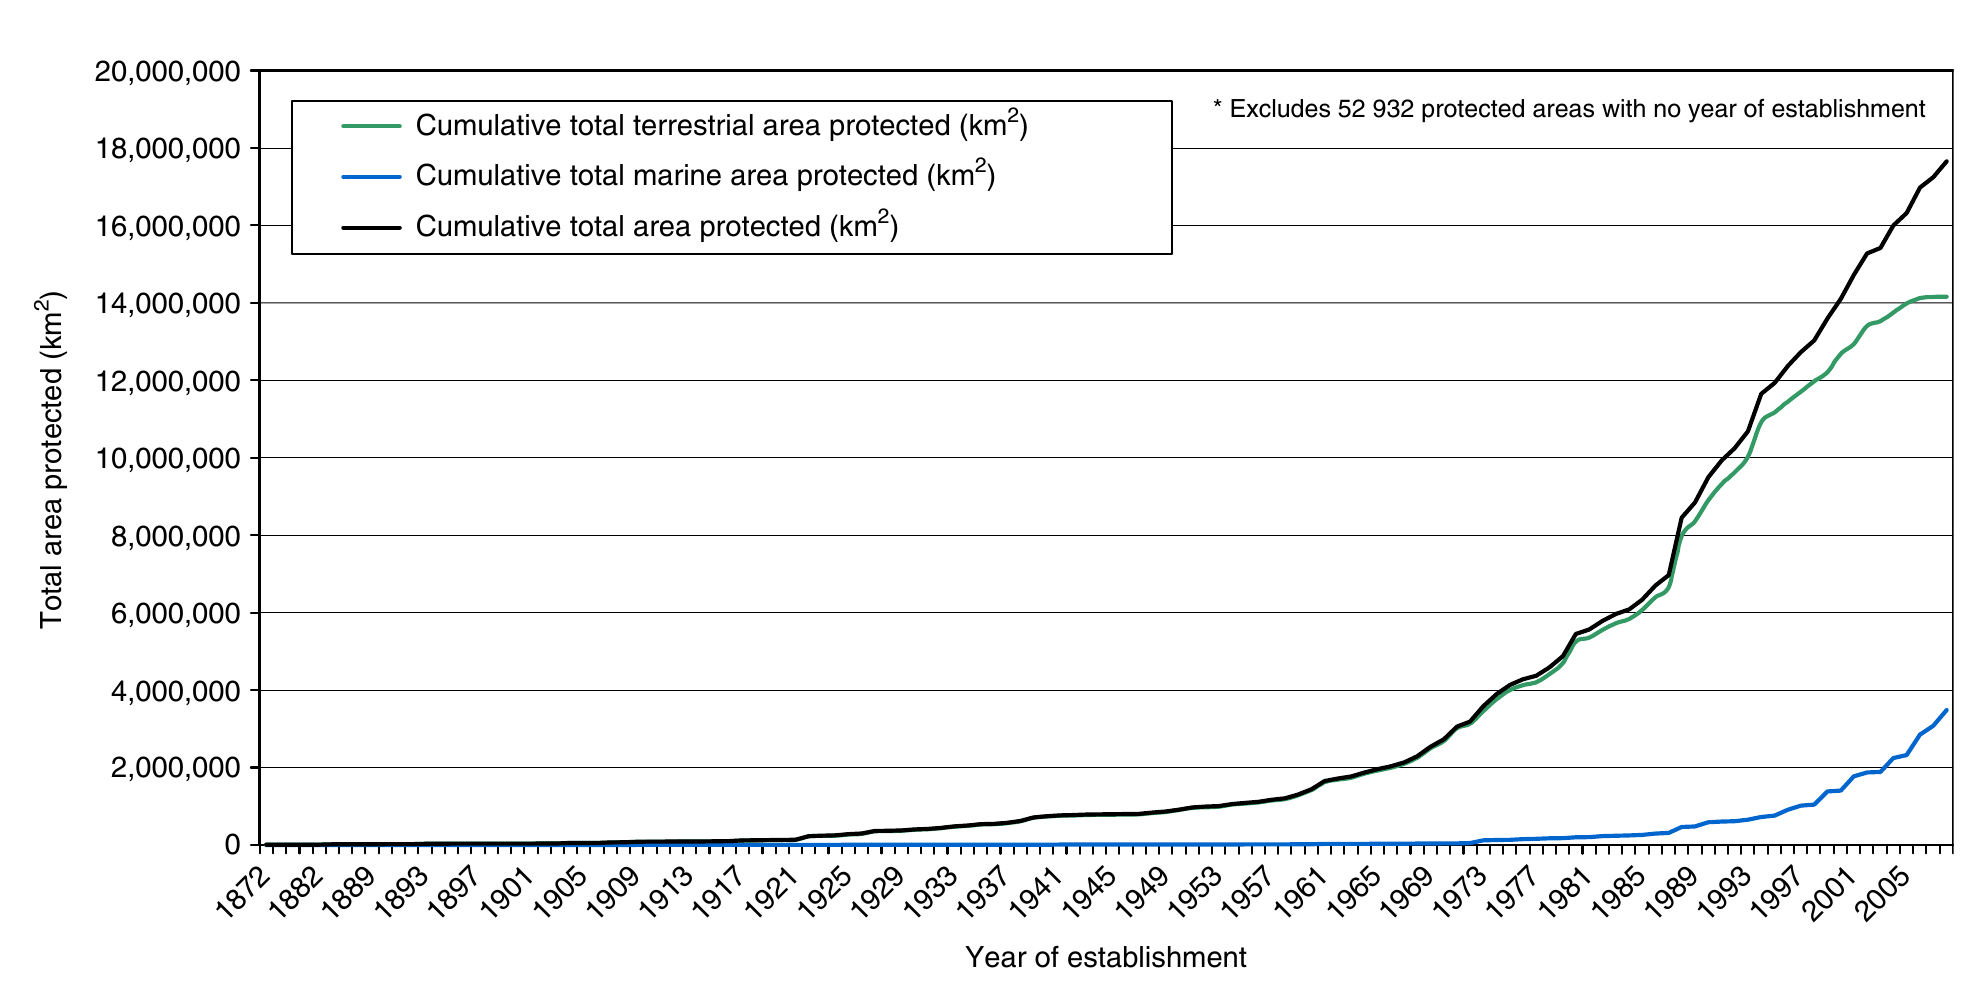
\includegraphics[width=0.65\linewidth]{./../images/global_protected_area} \caption{Global growth in protected areas. Reproduced from IUCN and UNEP-WCMC (2009).}\label{fig:global}
\end{figure}
\end{frame}

\begin{frame}{}
\protect\hypertarget{section-10}{}
\begin{figure}
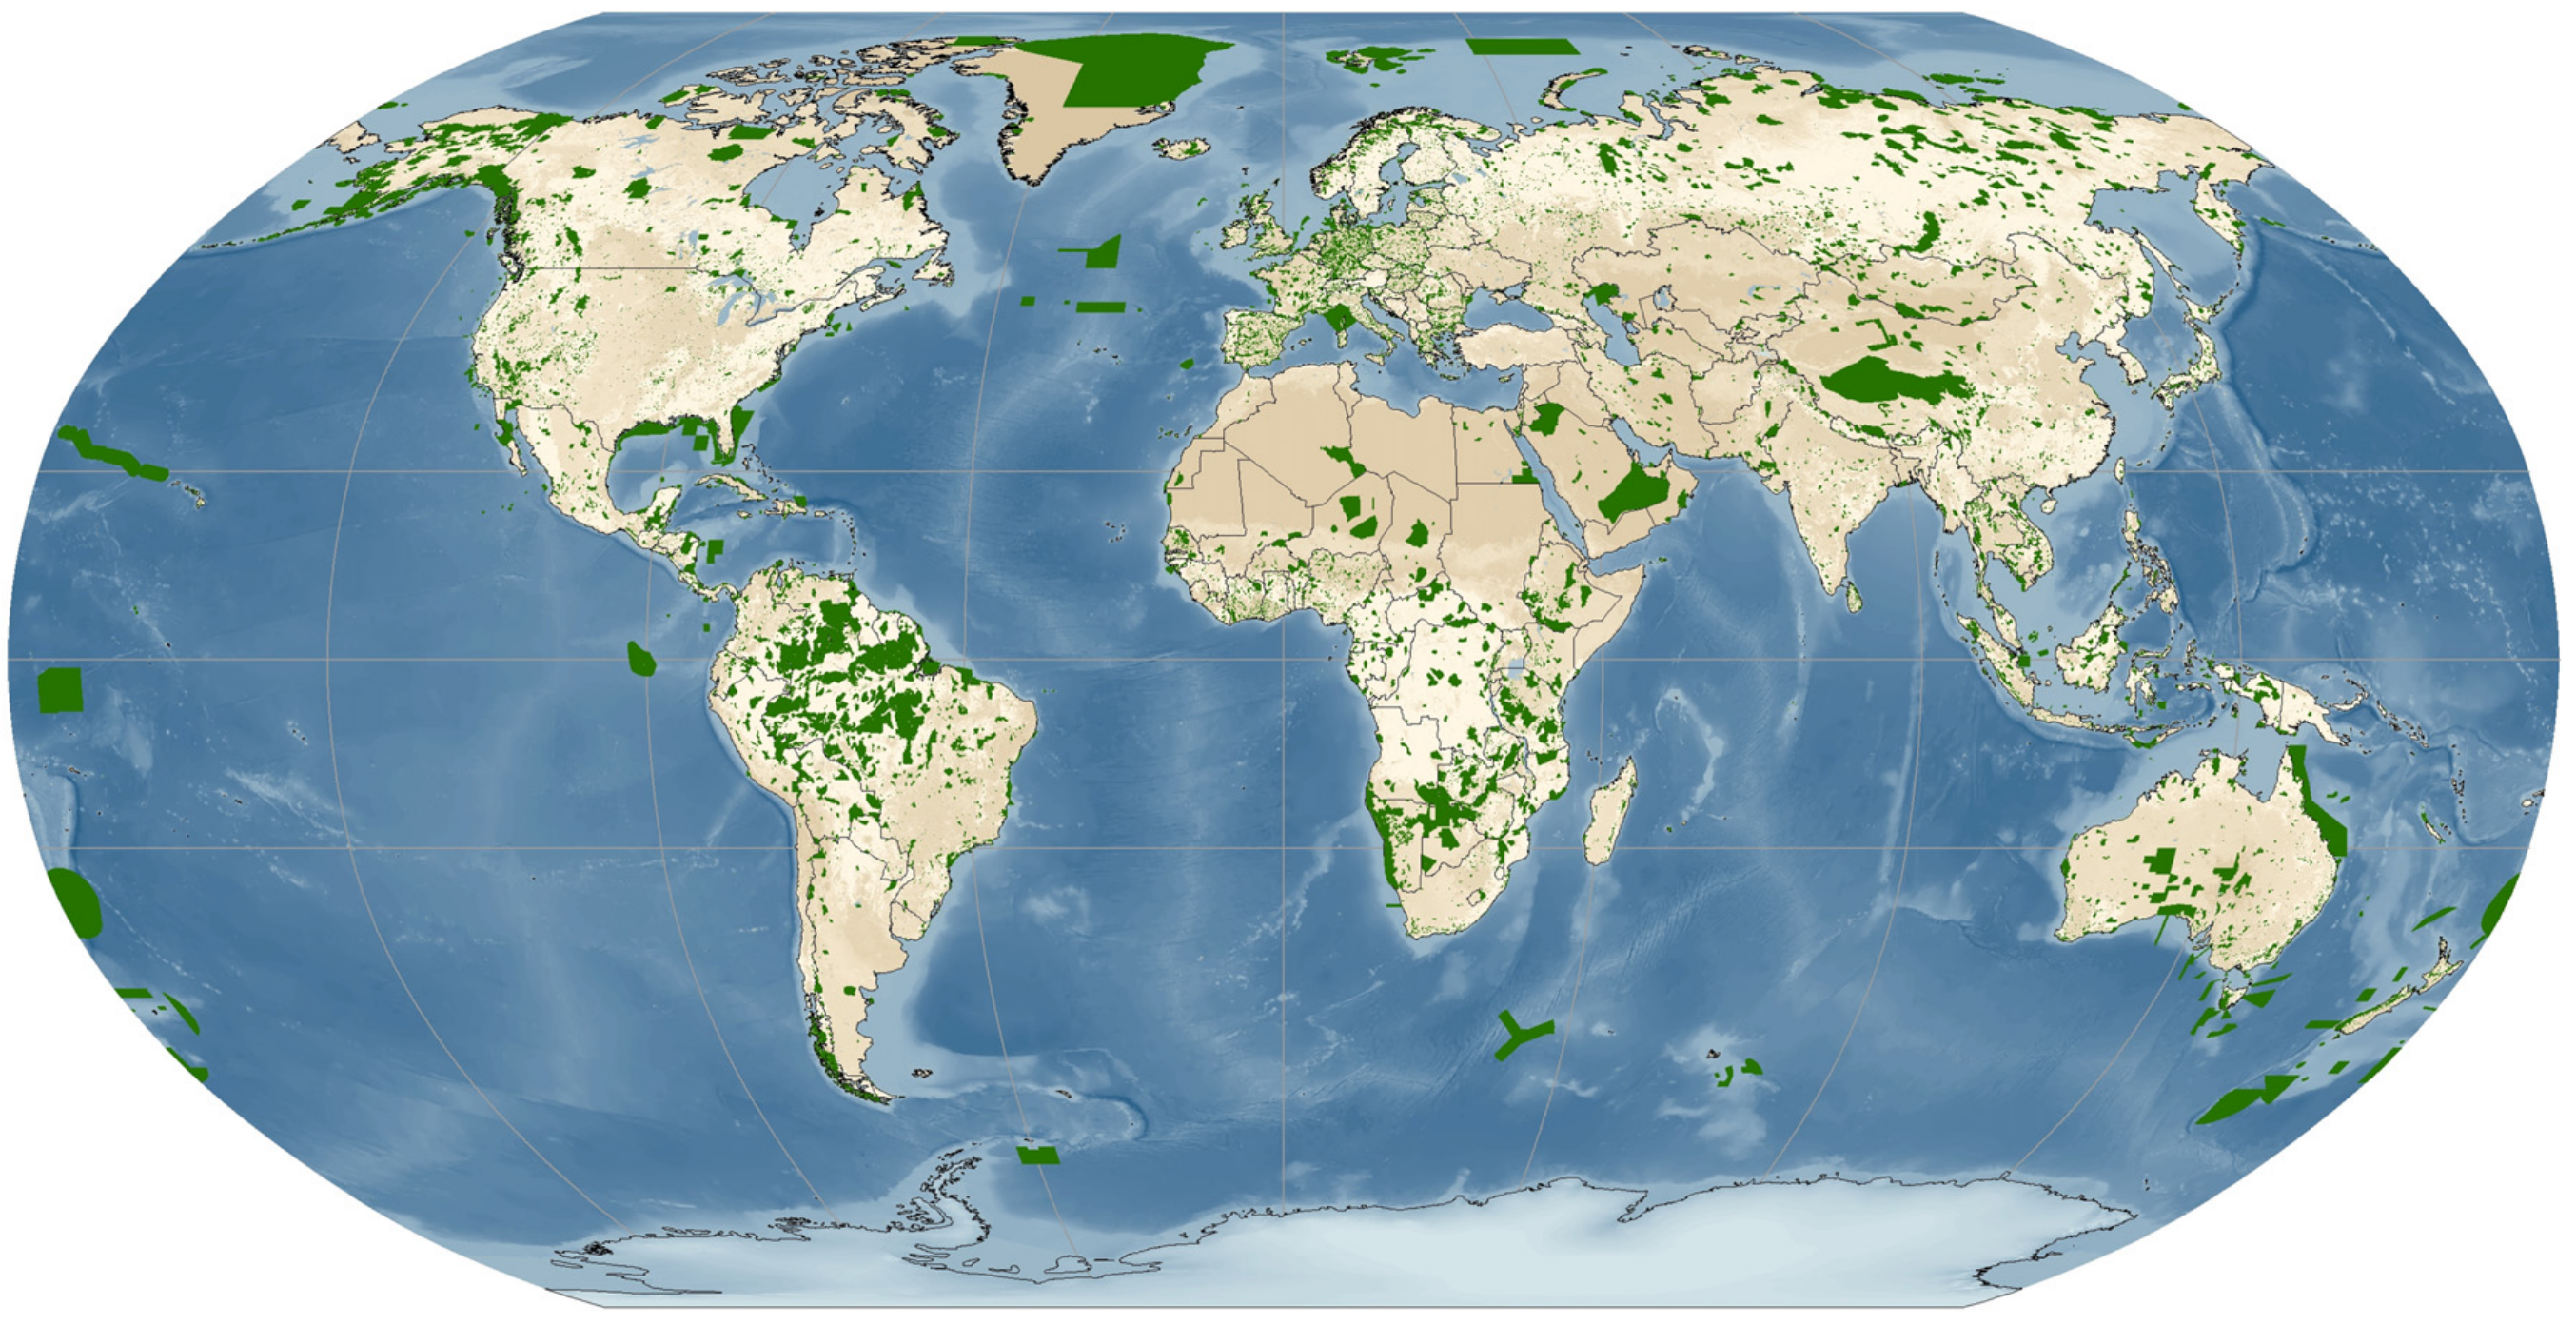
\includegraphics[width=0.8\linewidth]{./../images/global_protected_area_map} \caption{Protected areas of the world. Reproduced from World Database on Protected Areas (WDPA), UNEP-WCMC, July 2011.}\label{fig:global-map}
\end{figure}
\end{frame}

\begin{frame}{Protected area coverage of the world's biomes}
\protect\hypertarget{protected-area-coverage-of-the-worlds-biomes}{}
\begin{table}

\caption{\label{tab:unnamed-chunk-1}Protected area coverage of worlds biomes (in percentage)}
\centering
\fontsize{6}{8}\selectfont
\begin{tabular}[t]{lr}
\toprule
Biome & Percentage cover\\
\midrule
Tropical and subtropical moist broadleaf forests (TMF) & 5.5\\
Tropical and subtropical dry broadleaf forests (TDF) & 5.0\\
Tropical and subtropical coniferous forests (TCF) & 2.5\\
Temperate broadleaf and mixed forests (TeBF) & 3.8\\
Temperatre coniferous forests (TeCF) & 8.8\\
\addlinespace
Boreal forests/taiga (BF) & 6.2\\
Tropical and subtropical grasslands, savannas, and shrublands (TG) & 5.8\\
Temperate grasslands, savannas, and shrublands (TeG) & 2.0\\
Flooded grasslands and savannas (FG) & 8.8\\
Montane grasslands and shrublands (MG) & 3.8\\
\addlinespace
Tundra (T) & 13.8\\
Mediteranean forests, woodlands, and scrub or Sclerophyll forests (MF) & 3.0\\
Deserts and xeric shrublands (D) & 3.8\\
Mangrove (M) & 8.5\\
\bottomrule
\end{tabular}
\end{table}
\end{frame}

\begin{frame}{Protected areas nepal}
\protect\hypertarget{protected-areas-nepal}{}
\begin{table}

\caption{\label{tab:protected-areas-np1}Protected areas of Nepal}
\centering
\fontsize{5}{7}\selectfont
\begin{tabular}[t]{>{\raggedright\arraybackslash}p{8em}>{\raggedright\arraybackslash}p{5em}>{\raggedright\arraybackslash}p{5em}>{\raggedright\arraybackslash}p{6em}>{\raggedright\arraybackslash}p{40em}}
\toprule
Protected Area & Year Established & Area (sq. km.) & Elevation (m) & Conservation Significance\\
\midrule
\textbf{\cellcolor{gray!6}{1 Chitwan (World Heritage Site 1984)}} & \cellcolor{gray!6}{1973} & \cellcolor{gray!6}{932} & \cellcolor{gray!6}{150-815} & \cellcolor{gray!6}{The Park houses over 50 species of mammals including one-horned rhinoceros, Royal Bengal tiger and bison; Important Bird Area; 539 species of birds that include migrant birds like paradise flycatcher, Indian pitta, parakeets and several species of waterfowl; and many species of amphibians and reptiles including the endangered gharial, marsh mugger crocodile and python. The habitat comprises of deciduous broadleaf forest with over 600 plant species, savannas and wetlands.}\\
\textbf{2 Langtang} & 1976 & 1710 & 792-7,245 & The habitat types range from sub-tropical forests below 1,000 m to alpine shrubs and grasslands. Musk deer and red panda are at the focus of conservation. Many other mammals such as snow leopard, wild dog, Himalayan black bear, Himalayan tahr, ghoral, serow, rhesus monkey and langur monkey, and over 370 species of birds including tragopan and impeyan pheasant (danphe) are found.\\
\textbf{\cellcolor{gray!6}{3 Rara}} & \cellcolor{gray!6}{1976} & \cellcolor{gray!6}{106} & \cellcolor{gray!6}{1,800-4,048} & \cellcolor{gray!6}{Rara has many animal species including endangered red panda and musk deer. Three species of snow trout are found in the lake. During winter over 270 species of birds including coots, great-crested grebe, black-necked grebe, red crested pochard, mallard, common teal, merganser and gulls, and migrant water fowls can be seen. Coniferous forests, primarily of blue pine forms the dominant vegetation. Rhododendron, juniper, spruce, oak and cypress are found around 3,000 m while spruce and fir are more common at higher elevations.}\\
\textbf{4 Sagarmatha (World Heritage Site 1979)} & 1976 & 1148 & 2,800-8,848 & The Park is famous for the scenic beauty of the Himalayas (including Mount Everest), musk deer, red panda, beer and snow leopard. Nearly 200 species of birds including impeyan pheasant, blood pheasant, red-billed chough, yellow-billed chough, snow cock, and snow pigeon are found. The forest vegetation comprises of pine and hemlock forests at lower elevations, and silver fir, birch, rhododendron and juniper at higher elevations (i.e. above 3,500 m).\\
\textbf{\cellcolor{gray!6}{5 Shey-Phoksundo}} & \cellcolor{gray!6}{1984} & \cellcolor{gray!6}{3555} & \cellcolor{gray!6}{2,000-6,885} & \cellcolor{gray!6}{Wild goat (ghoral), blue sheep, musk deer, and the Shey-Phoksundo lake are some of the main attractions. Over 200 species of birds including yellow throated marten, Tibetan partridge, wood snipe, white-throated tit, wood accentor and crimson-eared rose finch, impeyan pheasant, cheer pheasant, chough, raven, Tibetan snow cock, Tibetan twit and Himalayan griffon; and 29 species of butterflies are found. Pine, walnut, willow, oak, cypress are dominant trees in the lower elevations and pine, spruce, juniper and birch at higher elevations. Alpine range is comprised of meadows and shrubs of berberis, wild rose and caragana.}\\
\bottomrule
\end{tabular}
\end{table}
\end{frame}

\begin{frame}{}
\protect\hypertarget{section-11}{}
\begin{table}

\caption{\label{tab:protected-areas-np2}Protected areas of Nepal (...continued)}
\centering
\fontsize{5}{7}\selectfont
\begin{tabular}[t]{>{\raggedright\arraybackslash}p{8em}>{\raggedright\arraybackslash}p{5em}>{\raggedright\arraybackslash}p{5em}>{\raggedright\arraybackslash}p{6em}>{\raggedright\arraybackslash}p{40em}}
\toprule
Protected Area & Year Established & Area (sq. km.) & Elevation (m) & Conservation Significance\\
\midrule
\textbf{\cellcolor{gray!6}{6 Khaptad}} & \cellcolor{gray!6}{1984} & \cellcolor{gray!6}{225} & \cellcolor{gray!6}{1,000-3,276} & \cellcolor{gray!6}{The Park is famous for medicinal plants. Over 220 species of medicinal plants are recorded. Wildlife includes barking deer, wild boar, ghoral, Himalayan black bear, yellow-throated marten, rhesus monkey and langur monkey, and around 270 species of birds are found. Vegetation is mainly comprised of grasslands and subtropical, temperate, and sub alpine forests. This is also a famous spiritual site}\\
\textbf{7 Bardia} & 1988 & 968 & 152-1,494 & Mammals such as Royal Bengal tiger, one-horned rhinoceros, elephant, swamp deer, black buck, and reptiles such as gharial, marsh mugger crocodile are the main species. Fresh-water Gangetic dolphin is found in the Karnali River. Bengal florican, lesser florican, silver-eared mesia and sarus crane are some of 400 species of birds found in the Park that is dominated by sal forest and savannahs.\\
\textbf{\cellcolor{gray!6}{8 Makalu Barun}} & \cellcolor{gray!6}{1991} & \cellcolor{gray!6}{1500} & \cellcolor{gray!6}{435-8,463} & \cellcolor{gray!6}{The park is an important habitat for endangered red panda and snow leopard, and several species of endangered plants. Above 80 varieties of fish including salmon are reported in the Arun River. Wren babbler and olive ground warbler are some of the 400 species of birds found in the Park. Forest vegetation ranges from sub-tropical forests to sub-alpine and alpine vegetation as the elevation increases. The park is also famous for Rhododendrons and orchids.Twenty-five (out of 30 found in Nepal) varieties of rhododendrons, 48 species of orchids, 87 species of medicinal herbs, 48 species o primroses and 86 species of fodder trees are reportedly found in the Park.}\\
\textbf{9 Shivapuri-Nagarjun} & 2002 & 159 & 1,366-2,732 & Conservation of watershed that drains the Kathmandu Valley is a major objective. Around 19 species of mammals including Himalayan black bear, leopard, barking deer, wild boar, wild cat, rhesus monkey and langur monkey, 177 species of birds, 102 species of butterflies, and 129 varieties of mushrooms are reported.\\
\textbf{\cellcolor{gray!6}{10 Banke}} & \cellcolor{gray!6}{2010} & \cellcolor{gray!6}{550} & \cellcolor{gray!6}{360-480} & \cellcolor{gray!6}{Conservation of endangered wildlife and strengthening of transboundary biological corridor are some of the main objectives. Includes eight natural ecosystems, and houses 124 species of plants, 34 mammals, more than 300 birds, 24 reptiles, seven amphibians, and 58 fish species}\\
\bottomrule
\end{tabular}
\end{table}
\end{frame}

\begin{frame}{}
\protect\hypertarget{section-12}{}
\begin{table}

\caption{\label{tab:protected-areas-np3}Protected areas of Nepal (...continued)}
\centering
\fontsize{5}{7}\selectfont
\begin{tabular}[t]{>{\raggedright\arraybackslash}p{8em}>{\raggedright\arraybackslash}p{5em}>{\raggedright\arraybackslash}p{5em}>{\raggedright\arraybackslash}p{6em}>{\raggedright\arraybackslash}p{40em}}
\toprule
Protected Area & Year Established & Area (sq. km.) & Elevation (m) & Conservation Significance\\
\midrule
\textbf{\cellcolor{gray!6}{1 Shuklaphanta}} & \cellcolor{gray!6}{1976} & \cellcolor{gray!6}{305} & \cellcolor{gray!6}{90-270} & \cellcolor{gray!6}{Major wildlife consists of swamp deer, wild elephant, tiger, several species of deer, wild boar, leopard, and monkeys. Marsh mugger crocodile, cobra, and python are Common reptiles.Important Bird Area; Saruscrane,swampfrancolin,grassowl, warblers, flycatchers, Bengal florican are the common birds found in the sub-tropical sal forest and open grasslands.}\\
\textbf{2 Koshi Tappu (Ramsar Site, 1987)} & 1976 & 175 & 80-100 & Wild buffalo and Siberian migratory birds are the main focus of conservation. Vegetation consists of grasslands with patches of scrub and deciduous riverine forests. Many other species of mammals (such as wild elephants, wild boar, hog deer, spotted deer, blue bull and jackal); Important Bird Area; 479 species of birds, and reptiles are found. Gangetic dolphins are found in the Koshi River.\\
\textbf{\cellcolor{gray!6}{3 Parsa}} & \cellcolor{gray!6}{1984} & \cellcolor{gray!6}{499} & \cellcolor{gray!6}{150-815} & \cellcolor{gray!6}{Wildlife species including wild elephant, tiger leopard, sloth bear, and gaur; reptiles including king cobra, common cobra, krait, rat snake and python; over 370 species of birds including the endangered great hornbill are reported. Natural vegetation consists of tropical and sub-tropical sal forests. Chir pine, khair, and sissoo trees are found on the hilly parts.}\\
\textbf{1 Dhorpatan} & 1987 & 1325 & 2,850-7,000 & The reserve is famous for blue sheep, which is open for regulated trophy hunting\\
\textbf{\cellcolor{gray!6}{1 Annapurna}} & \cellcolor{gray!6}{1992} & \cellcolor{gray!6}{7629} & \cellcolor{gray!6}{1,000-8,092} & \cellcolor{gray!6}{Endemic plants and mountains are the main characteristics. Over 100 species of mammals including blue sheep and endangered snow leopard; 39 species of reptiles; 22 species of amphibians; Important Bird Area (IBA); 474 species of birds including multi-colored impeyan pheasant, kokla and blood pheasant are reported. Many species of orchids and rhododendrons are found.}\\
\bottomrule
\end{tabular}
\end{table}
\end{frame}

\begin{frame}{}
\protect\hypertarget{section-13}{}
\begin{table}

\caption{\label{tab:protected-areas-np4}Protected areas of Nepal (...continued)}
\centering
\fontsize{5}{7}\selectfont
\begin{tabular}[t]{>{\raggedright\arraybackslash}p{8em}>{\raggedright\arraybackslash}p{5em}>{\raggedright\arraybackslash}p{5em}>{\raggedright\arraybackslash}p{6em}>{\raggedright\arraybackslash}p{40em}}
\toprule
Protected Area & Year Established & Area (sq. km.) & Elevation (m) & Conservation Significance\\
\midrule
\textbf{\cellcolor{gray!6}{2 Kanchanjunga}} & \cellcolor{gray!6}{1997} & \cellcolor{gray!6}{2035} & \cellcolor{gray!6}{1,200-8,598} & \cellcolor{gray!6}{Mammals including endangered snow leopard, Himalayan black bear, musk deer, red panda, blue sheep, rhesus monkey; 252 species of different birds including impeyan pheasant, red-billed blue magpie, ashy drongo; 20 indigenous gymnosperms, 15 among Nepal's 23 endemic flowering plants, 30 varieties of rhododendrons and 48 varieties of orchids are reported.}\\
\textbf{3 Manasula} & 1998 & 1663 & 1,360-8,163 & Snow leopard, musk deer and Himalayan Tahr are among the 33 species of mammals found in the conservation area. Over 110 species of birds and 1,500-2,000 species of flowering plants are reported.\\
\textbf{\cellcolor{gray!6}{5 Khairapur}} & \cellcolor{gray!6}{2010} & \cellcolor{gray!6}{16} & \cellcolor{gray!6}{120-230} & \cellcolor{gray!6}{The first organized effort to conserve the endangered blackbuck (Antilope cervicapra).}\\
\textbf{6 Api Nampa} & 2010 & 1903 & 539-7,132 & Snow leopard, musk deer, clouded leopard, ghoral, Himalayan black bear and Himalayan tahr are found in the area.\\
\bottomrule
\end{tabular}
\end{table}
\end{frame}

\begin{frame}{Framework for reviewing contribution}
\protect\hypertarget{framework-for-reviewing-contribution}{}
\begin{figure}
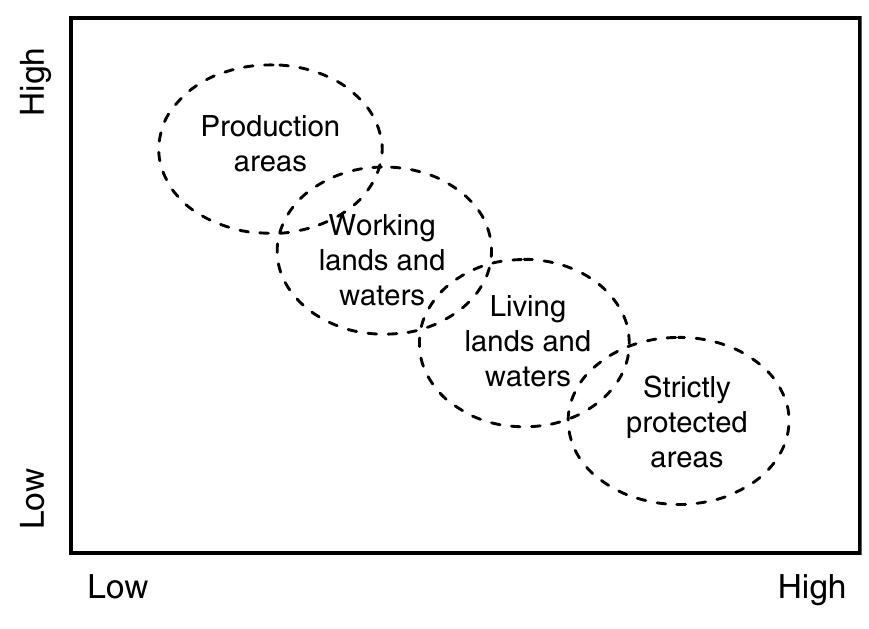
\includegraphics[width=0.45\linewidth]{./../images/contribution_review} \caption{A framework for reviewing the contribution of areas of land and water to biodiversity conservation. Starting at the bottom right hand corner the framework moves from 'strictly protected areas', reflecting the more traditional approach to protected areas managed almost exclusively for biodiversity conservation, The next category is 'living lands and waters', which are areas managed primarily for biodiversity conservation with some extractive uses limited to the ecologically sustainable management of areas of land and water to support life of all forms. 'Working lands and waters' are mostly agricultural lands managed primarily for extractive uses while attempting to conserve biodiversity at the same time. The final category is 'production areas' of land and water where the management focuses exclusively on maximizing extractive and productive uses and biodiversity conservation is not an objective.}\label{fig:contribution-review}
\end{figure}
\end{frame}

\hypertarget{methods-of-biodiversity-conservation}{%
\section{Methods of biodiversity
conservation}\label{methods-of-biodiversity-conservation}}

\begin{frame}{}
\protect\hypertarget{section-14}{}
\begin{enumerate}
\tightlist
\item
  \emph{In situ} conservation;
\item
  \emph{Ex situ} conservation
\item
  Restoration
\end{enumerate}
\end{frame}

\hypertarget{area-specificlocal-approach}{%
\section{Area-specific/local
approach}\label{area-specificlocal-approach}}

\begin{frame}{Farmer as pivot}
\protect\hypertarget{farmer-as-pivot}{}
\begin{itemize}
\tightlist
\item
  Which crop I can cultivate ?
\item
  Which varieties perform good on my locality ?
\item
  Which variety yields better ?
\item
  Which variety can escape disease well ?
\item
  Which crop or crop mixtures are likely to perform well in which season
  ?
\item
  What seed do I store for the upcoming crop ?
\item
  How do I best manage my land to have a good harvest ?
\item
  How do I best preserve the seed to ensure good planting ?
\item
  How do mix or relay my collection of crops where I grow ?
\item
  How do I preserve the integrity of a good variety ?
\end{itemize}
\end{frame}

\begin{frame}{Institutional conservation approaches}
\protect\hypertarget{institutional-conservation-approaches}{}
\begin{itemize}
\tightlist
\item
  Single species based conservation. For e.g.~\emph{Ex situ}
  conservation for single species (e.g., zoos, expensive reintroduction
  programs, captive breeding programs).
\item
  Umbrella species approach
\item
  Elimination of invasise species linked to conservation failures.
\item
  Protected areas management, for human exclusion.
\item
  Fragmentation and loss of ecosystem management through management of
  spatial distribution of ecosystem or habitats.
\item
  Incorporation of short-frequency disturbances.
\item
  Limitting or excluding human extraction of resources from nature
  reserves.
\item
  Reserve design and size allocation based on territory need of each
  species.
\item
  Use of corridors and buffer zones to link habitat fragments and
  reserve networks.
\item
  Small-scale, data-intensive species and community model design and
  implementation.
\item
  Development of nonmarket values for species.
\end{itemize}
\end{frame}

\hypertarget{national-nepalsregional-approaches}{%
\section{National (Nepal's)/regional
approaches}\label{national-nepalsregional-approaches}}

\begin{frame}{Targeted/sectoral approach}
\protect\hypertarget{targetedsectoral-approach}{}
\begin{enumerate}
\tightlist
\item
  Management of protected areas
\end{enumerate}

\begin{itemize}
\tightlist
\item
  A: Improvement in management of protected areas and species.
\item
  B: Abatement in poaching and illegal trade of wildlife and wildlife
  parts
\item
  C: Improvement in protected area habitats and connectivity
\item
  D: Improvement in management of protected area tourism
\end{itemize}

\begin{enumerate}
\setcounter{enumi}{1}
\tightlist
\item
  Management of biodiversity outside protected area
\end{enumerate}

\begin{itemize}
\tightlist
\item
  A: Improvement in forest governance and management
\item
  B: Significant reduction (by at least 75\% of the current rate) in the
  loss and degradation of forest
\item
  C: Improvement in conservation of biodiversity in community managed
  forests
\item
  D: Enhancing conservation of species and genetic diversity
\item
  F: Enhancing forest based livelihoods
\end{itemize}
\end{frame}

\begin{frame}{Targeted/sectoral approach (\ldots continued)}
\protect\hypertarget{targetedsectoral-approach-continued}{}
\begin{enumerate}
\setcounter{enumi}{2}
\tightlist
\item
  Management of rangeland biodiversity
\item
  Management of watershed biodiversity
\item
  Management of agrobiodiversity
\item
  Management of mountain biodiversity
\end{enumerate}
\end{frame}

\begin{frame}{Cross-thematic and cross-sectoral strategies}
\protect\hypertarget{cross-thematic-and-cross-sectoral-strategies}{}
\begin{itemize}
\tightlist
\item
  Addressing the policy and legislative gaps
\item
  Institutional strengthening
\item
  Mainstreaming biodiversity across the government, society and economy
\item
  Harmonization of biodiversity related international conventions
\item
  Enhancement of national capacity for improved management of
  biodiversity
\item
  Landscape management
\item
  Management of invasive alien species
\item
  Adaptation to and mitigation of the effects of climate change
\item
  Integrating gender and social inclusion perspectives
\end{itemize}
\end{frame}

\begin{frame}{Cross-thematic (\ldots continued)}
\protect\hypertarget{cross-thematic-continued}{}
\begin{itemize}
\tightlist
\item
  Conservation of and Respect to Traditional Knowledge, Innovations and
  Practices of Indigenous and Local Communities
\item
  Knowledge generation and management
\item
  Technology development, acquisition and use
\item
  Communication, extension and outreach
\item
  Fund generation and mobilization
\item
  Monitoring evaluation and reporting
\end{itemize}
\end{frame}

\hypertarget{international-convention-and-treaties}{%
\section{International convention and
treaties}\label{international-convention-and-treaties}}

\hypertarget{intellectual-property-rights}{%
\section{Intellectual property
rights}\label{intellectual-property-rights}}

\begin{frame}{Background}
\protect\hypertarget{background-1}{}
\begin{itemize}
\tightlist
\item
  IP protection consists of principles that a society observes to ensure
  that an inventor is protected from the unfair use of his/her invention
  by others.
\item
  Protection is provisioned in the form of:

  \begin{itemize}
  \tightlist
  \item
    Copyright
  \item
    Patent
  \item
    Trademark
  \item
    Trade secret
  \item
    Breeder's right
  \item
    Confidential information
  \end{itemize}
\item
  Innovation has a price tag, hence the investor must be compensated
\item
  Ensures that invention is not kept secret from betterment of society.
\item
  Law and science meet here.
\end{itemize}
\end{frame}

\begin{frame}{Guiding treaties, agreements and institutions}
\protect\hypertarget{guiding-treaties-agreements-and-institutions}{}
\begin{itemize}
\tightlist
\item
  Agreement on Trade related Aspects of Intellectual Property Rights
  (TRIPS Agreement) within the World Trade Organization (WTO) in 1995
  (effective since).
\item
  International Treaty on Plant Genetic Resources for Food and
  Agriculture in (ITPGRFA) 2002.
\item
  World Intellectual Property Organization
  (\href{https://www.wipo.int/portal/en/index.html}{WIPO})
\item
  International Union for the Protection of New Varieties of Plants
  (Union International pour la Protection des Obtentions Vegetales;
  UPOV) established in 1961.
\end{itemize}
\end{frame}

\begin{frame}{Traditional knowledge}
\protect\hypertarget{traditional-knowledge}{}
\begin{itemize}
\tightlist
\item
  Association between level of biodiversity in a specific region with
  cultural distinctiveness of its inhabitants.
\item
  Specific knowledge of communities living in close relationship to
  their environment: traditional knowledge.
\item
  Integrated into

  \begin{itemize}
  \tightlist
  \item
    Rio Process,
  \item
    International Treaty on PGRFA
  \item
    \href{https://sustainabledevelopment.un.org/milesstones/wssd}{World
    Summit on Sustainable Development}; Johannesburg, South Africa 26
    August - 4 September 2002.
  \end{itemize}
\item
  CBD speaks of `traditional knowledge, innovations and practices of
  indigenous and local communities embodying traditional lifestyles
  relevant for the conservation and sustainable use of biological
  diversity' (Article 8(j)).
\end{itemize}
\end{frame}

\begin{frame}{Traditional knowledge}
\protect\hypertarget{traditional-knowledge-1}{}
\begin{itemize}
\tightlist
\item
  Foster sharing of economic incentives to making available traditional
  knowledge, to conserve it through use, and thereby enhance the
  livelihoods of farming and indigenous communities and reverse the
  decline of biodiversity, upon which, in return, long-term food
  security is based. \citep{biber2006rights}
\item
  Since the adoption of convention on Biological Diversity (CBD) in
  1992, the law of plant genetic resources (PGR) and the legal status of
  traditional knowledge (TK) has attracted increasing attention.
\item
  2001 Doha Agenda of the WTO explicitly endorsed the issue of
  traditional knowledge as a subject for further work.
\end{itemize}
\end{frame}

\begin{frame}{Traditional knowledge}
\protect\hypertarget{traditional-knowledge-2}{}
\begin{itemize}
\tightlist
\item
  TK has common features for both indigenous as well as farming
  communities:

  \begin{itemize}
  \tightlist
  \item
    Information is not an individual creation, but the achievement of a
    specific community.
  \item
    It cumulates over many generations and evolve accordingly.
  \item
    Managed by and exchanged through customs or customary laws.
  \item
    Close interaction exists between TK and the surrounding ecosystem.
  \end{itemize}
\end{itemize}
\end{frame}

\begin{frame}{Farmer's right}
\protect\hypertarget{farmers-right}{}
\begin{itemize}
\tightlist
\item
  Intellectual contribution of farmers to the diversity of crop
  varieties and animal breeds emphasized in `Farmers' Rights Charter', a
  document drafted by Indian Farmers' Unions.
\item
  Guiding thoughts:

  \begin{itemize}
  \tightlist
  \item
    Farmers ought to have the right to `participate fully in any
    benefits derived from the improved use of these genetic resources'
    and, of course, in the ITPGRFA (Preamble para. 7 and Article 9.1).
  \item
    Farmers' innovations take place collectively and cumulatively, and
    that therefore farmers' rights, arising from their role as
    conservators and breeders, are community rights.
  \end{itemize}
\end{itemize}
\end{frame}

\begin{frame}{UPOV}
\protect\hypertarget{upov}{}
\small

\begin{itemize}
\tightlist
\item
  It seeks to protect new varieties of plants both in the interest of
  agricultural development and of plant breeders.
\item
  UPOV sought from the outset to provide incentives to the private
  sector to engage in commercial plant breeding, by introducing
  so-called plant breeders' rights, aka. Plant Variety Rights.
\item
  Agreed guidelines for the conduct of tests and standardization of
  variety descriptions based upon the morphology of the grain and plant.
\item
  PBR is an IPR, often described as plant ``patent''. Breeders can claim
  royalties on seed sold.
\item
  Once granted, PBR ecognizes the exclusive rights of individual plant
  breeders to produce or reproduce protected varieties, to condition
  them for the purpose of propagation, to offer them for sale, to
  commercialize them, including exporting and importing them, and to
  stock them with a view to production or commercialization (Article
  14.1 UPOV).
\item
  Like any patent right, PBR expires after 20 years.
\end{itemize}
\end{frame}

\begin{frame}{TRIPS}
\protect\hypertarget{trips}{}
\begin{itemize}
\tightlist
\item
  General Agreement on Tariffs and Trade (GATT) contains important
  provisions covering the protection of intellectual property in the
  agreement on Trade Related Aspects of Intellectual Property Rights
  (TRIPS).
\item
  For most member countries ratification of GATT means membership of
  UPOV and a PBR system based upon plant morphology.
\item
  Plant breeders will still use morphological characters to purify
  candidate varieties before submitting them for tests and trials, and
  seed traders will still use morphological characters to verify variety
  at the point of sale.
\item
  However, the science of systematics is being revolutionized by
  molecular technologies.
\item
  Concept of ``Essentially derieved varieties''
\end{itemize}
\end{frame}

\renewcommand\refname{Bibliography}
\begin{frame}[allowframebreaks]{Bibliography}
  \bibliographytrue
  \bibliography{../bibliography/bibliographies.bib}
\end{frame}

\end{document}
